  \documentclass[final]{beamer} % beamer 3.10: do NOT use option hyperref={pdfpagelabels=false} !
  %\documentclass[final,hyperref={pdfpagelabels=false}]{beamer} % beamer 3.07: get rid of beamer warnings
  \mode<presentation> {  %% check http://www-i6.informatik.rwth-aachen.de/~dreuw/latexbeamerposter.php for examples
    \usetheme{UW}    %% you should define your own theme e.g. for big headlines using your own logos 
  }
  \newlength{\mylength}
\usepackage{ragged2e}

  \usepackage[english]{babel}
  \usepackage[latin1]{inputenc}
  \usepackage{amsmath,amsthm, amssymb, latexsym}
  %\usepackage{times}\usefonttheme{professionalfonts}  % times is obsolete
  \usefonttheme[onlymath]{serif}
  \boldmath
  \usepackage[orientation=landscape,size=a0,scale=1.4,debug]{beamerposter}                       % e.g. for DIN-A0 poster
  %\usepackage[orientation=portrait,size=a1,scale=1.4,grid,debug]{beamerposter}                  % e.g. for DIN-A1 poster, with optional grid and debug output
  %45'' wide, 35'' high
  
  %\usepackage[orientation=portrait,size=a0,scale=1.0,printer=rwth-glossy-uv.df]{beamerposter}   % e.g. for DIN-A0 poster with rwth-glossy-uv printer check
  % ...
  %\usepackage
  \usepackage{xspace}
  \usepackage{tikz}
\usepackage{subfig}
  \usepackage{logictools}
\usepackage{prooftheory}
\usepackage{comment}
\usepackage{mathenvironments}
\usepackage{drawproof}
\usepackage{bussproofs}
\EnableBpAbbreviations

\usepackage{tensor}
\usepackage{mathtools}
\usepackage{amsmath}
\usepackage{commands}
  \title[Partial Regularization]{Partial Regularization of First-Order Resolution
Proofs}
  \author[Gorzny]{Jan Gorzny  \hspace{5cm}jgorzny@uwaterloo.ca}
  \institute[U. Waterloo]{School of Computer Science, University of Waterloo\\Supported by the Google Summer of Code Program 2014}
  \date{NASSLLI 2016}
  \setbeamertemplate{navigation symbols}{}

  \begin{document}
  \begin{frame}{} 
  \begin{columns}


  \begin{column}{0.3\textwidth}
      \vfill
      \begin{block}{Introduction}
       \justify %do not remove
       \begin{itemize}
       \item As the ability of automated deduction has improved, %to solve complex problems, 
it has been applied to new application domains; e.g. Furbach et al. \cite{furbach2015automated} used it in natural language reasoning. 
       \item  Resolution proof production is a key feature of modern theorem provers; the best, most-efficient provers do not necessarily generate the best, least redundant proofs.
       \item For proofs using propositional resolution generated by SAT- and SMT-solvers, there are many proof compression techniques. 
       
              \item One approach to compressing first-order logic proofs is to lift ideas used in propositional logic.
       \end{itemize}

    \end{block}
    
    \begin{block}{Propositional RecyclePivotsWithIntersection \cite{LURPI}}
    \begin{itemize}
\item Traverse a proof from the bottom up: store for every node a set of \emph{safe literals}: literals resolved in all paths below the node
\item For any node whose resolved literals are safe, replace it with one of its parents (\alert{\emph{regularizing} it}.)
\end{itemize}
The set of safe literals for a node $\eta$ will be denoted $\mathcal{S}(\eta)$.
\end{block}

      \begin{block}{A Propositional Example}
Consider the proof $\psi$ shown below:
\vspace{-10pt}
\begin{footnotesize}
\begin{prooftree}
\AXC{$ \eta_1 $}
		\AXC{$ \eta_2: a, c, \neg b $}
				\AXC{$ \eta_1: \neg a$}
						\AXC{$ \eta_3:  a, b $} \RName{$a$}
					\BIC{$ \eta_4: b$} \RName{$b$}
			\BIC{$ \eta_5: a, c$}	\RName{$a$}
	\BIC{$\eta_6: c$}
		\AXC{$ \eta_4 $}
				\AXC{$ \eta_7: a, \neg b, \neg c $} \RName{$b$}
			\BIC{$ \eta_8: a, \neg c$}	\RName{$c$}
					\AXC{$ \eta_1 $}  \RName{$a$}
				\BIC{$ \eta_9: \neg c$}	\RName{$c$}
		\BIC{$\psi: \bot$}	
\end{prooftree}
\end{footnotesize}

%The node $\eta_4$ has pivot $a$, left (right) resolved literal $\neg a$ ($a$). Its conclusion is $\{b\}$ and its premises are the conclusions of its parents: the input nodes $\eta_1$ ($\{ \neg a \}$) and $\eta_3$ ($\{ a, b\} $). It has two children ($\eta_5$ and $\eta_8$). 

%These observations lead to the idea of traversing the proof in a bottom-up manner, storing for every node a set of \emph{safe literals} that get resolved in all paths below it in the proof (or that already occurred in the root clause of the original proof). Moreover, if one of the node's resolved literals belongs to the set of safe literals, then it is possible to regularize the node by replacing it by one of its parents (cf.\ Algorithm~\ref{algo:RPI}). 
%Propositional RecyclePivotsWithIntersection:
%\begin{itemize}
%\item Traverse a proof from the bottom up: store for every node a set of \emph{safe literals}: literals resolved in all paths below the node
%\item For any node whose resolved literals are safe, replace it with one of its parents.
%\end{itemize}

%The regularization of a node should replace a node by one of its parents, and more precisely by the parent whose clause contains the resolved literal that is safe. After regularization, all nodes below the regularized node may have to be fixed. However, since the regularization is done with a bottom-up traversal, and only nodes below the regularized node need to be fixed, it is again possible to postpone fixing and do it with only a single traversal afterwards. 

The algorithm {\RPI} assigns $\mathcal{S}(\eta_5) \leftarrow \{a,c\}$, $\mathcal{S}(\eta_8)\leftarrow \{a, \neg c\}$, and
% as the safe literals of, respectively, $\eta_5$ and $\eta_8$. 
%The safe literals of $\eta_4$ w.r.t. its children $\eta_5$ and $\eta_8$ are respectively $\{a,c,b\}$ and $\{a, \neg c, b\}$, and hence the safe literals of $\eta_4$ are $\{a,b\} = \{a,c,b\}\cap \{ a,\lnot c, b\}$.
$\mathcal{S}(\eta_4) \leftarrow \{a,c,b\}\cap \{ a,\lnot c, b\} =  \{a,b\}$.
% Since the right resolved literal of $\eta_4$ ($a$) belongs to $\eta_4$'s safe literals, $\eta_4$ is correctly detected as a redundant node and hence regularized: $\eta_4$ is replaced by its right parent $\eta_3$. The resulting proof is shown below:
Since $a\in \mathcal{S}(\eta_4)$ where $a$ is a pivot of $\eta_4$, $\eta_4$ is detected as a redundant node and regularalized by replacing it by its right parent $\eta_3$:

\begin{small}
\begin{prooftree}
\AXC{$ \eta_1: \neg a $}
		\AXC{$ \eta_2: a, c, \neg b $}
						\AXC{$ \eta_3:  a, b $}\RName{$ $}
			\BIC{$ \eta_5: a, c$}	\RName{$ $}
	\BIC{$\eta_6: c$}
		\AXC{$ \eta_3 $}
				\AXC{$ \eta_7: a, \neg c, \neg b $} \RName{$ $}
			\BIC{$ \eta_8: a, \neg c$}	\RName{$ $}
					\AXC{$ \eta_1 $}  \RName{$ $}
				\BIC{$ \eta_9: \neg c$}	\RName{$ $}
		\BIC{$\psi: \bot$}	
\end{prooftree}
\end{small}

    \end{block}
          
      \begin{block}{A First-Order Example}
%straightforward example

%Consider the following proof $\psi$. 
Consider the proof $\psi$ below. When computed as in the propositional case, $\mathcal{S}(\eta_3) \leftarrow \{ \vdash q(c), ~ p(a,X)\}$


\begin{footnotesize}
\begin{prooftree}
\def\e{\mbox{\ $\vdash$\ }}
\AxiomC{$\eta_1$: \e $p(W,X)$}
\AxiomC{$\eta_2$: $p(W,X)$ \e $q(c)$}
\BinaryInfC{$\eta_3$: \e $q(c)$}
\AxiomC{$\eta_4$: $q(c)$ \e $p(a,X)$}
\BinaryInfC{$\eta_5$: \e $p(a,X)$}
\AxiomC{$\eta_6$: $p(Y,b)$ \e }
\BinaryInfC{$\psi$: $\bot$}
\end{prooftree}
\end{footnotesize}

\noindent
Since $p(W,X)\neq p(a,X)$, propositional {\RPI} algorithm would not change $\psi$. However, $\eta_3$'s left pivot $p(W,X)\in \eta_1$ is unifiable with the safe literal $p(a,X)$. Regularizing $\eta_3$, by deleting the edge between $\eta_2$ and $\eta_3$ and replacing $\eta_3$ by $\eta_1$, leads to further deletion of $\eta_4$ (because it is not resolvable with $\eta_1$) and finally to the following proof:


\begin{prooftree}
\def\e{\mbox{\ $\vdash$\ }}
\AxiomC{$\eta_1$: \e$p(W,X)$}
\AxiomC{$\eta_6$: $p(Y,b)$\e}
\BinaryInfC{$\psi'$: $\bot$}
\end{prooftree}


\noindent
%This example above suggests that, in the first-order case, it might suffice that a pivot be unifiable with a safe literal. However, there are cases, as shown in the next example, where mere unifiability is not enough and greater care is needed.
%\alert{Is unifiability enough?} The next examples show that this is not the case.
    \end{block}
    
    
        \vfill
  \end{column}
  
  \begin{column}{0.3\textwidth}
      \vfill
      \begin{block}{Unifiability is Not Enough}
    Consider $\psi$ below. When computed as in the propositional case, $\mathcal{S}(\eta_3)\leftarrow \{ \vdash q(c), ~ p(a,X)\}$, and as the pivot $p(a,c)$ is unifiable with the safe literal $p(a,X)$, $\eta_3$ appears to be a candidate for regularization. 

\begin{small}
\begin{prooftree}
\def\e{\mbox{\ $\vdash$\ }}
\AxiomC{$\eta_1$: \e $p(a,c)$}
\AxiomC{$\eta_2$: $p(a,c)$ \e $q(c)$}
\BinaryInfC{$\eta_3$: \e $q(c)$}
\AxiomC{$\eta_4$: $q(c)$ \e $p(a,X)$}
\BinaryInfC{$\eta_5$: \e $p(a,X)$}
\AxiomC{$\eta_6$: $p(Y,b)$ \e }
\BinaryInfC{$\psi$: $\bot$}
\end{prooftree}
\end{small}


\noindent
However, if we attempt to regularize the proof, the same series of actions as in the last example would 
require resolution between $\eta_1$ and $\eta_6$, which is not possible.
\end{block}
      \begin{block}{Pre-Regularization Unifiability}

Let $\eta$ be a node with pivot $\ell'$ unifiable with safe literal $\ell$ which is resolved against literals $\ell_1$, \ldots, $\ell_n$ in a proof $\psi$. $\eta$ is said to satisfy the \emph{pre-regularization unifiability property} in $\psi$ if $\ell_1$,\ldots,$\ell_n$, and $\dual{\ell'}$ are unifiable.
    \end{block}
    \begin{block}{Pre-Regularization Unifiability: Still Not Enough}
    %Satisfying the pre-regularization unifiability property is not sufficient. 
    Consider the proof $\psi$ below. After collecting the safe literals, $\mathcal{S}(\eta_3)\leftarrow \{q(T,V),p(c,d)\vdash q(f(a,e),c)\}$.

\begin{scriptsize}
\begin{prooftree}
\def\e{\mbox{\ $\vdash$\ }}
\AxiomC{$\eta_8$: $q(f(a,e),c)\e$\hspace{-1cm}}
\AxiomC{$\eta_6$: $\e p(c,d)$\hspace{-4.5cm}}
\AxiomC{$\eta_1$: $p(U,V)\e q(f(a,V),U)$}
\AxiomC{$\eta_2$: $q(f(a,X),Y),q(T,X)\e q(f(a,Z),Y)$}
\BinaryInfC{$\eta_3$: $p(U,V),Q(T,V)\e q(f(a,Z),U)$\hspace{-2cm}}
\AxiomC{\hspace{-3cm} $\eta_4$: $\e q(R,S)$}
\BinaryInfC{$\eta_5$: $p(U,V)\e q(f(a,Z),U)$}
\BinaryInfC{$\eta_7$: $\e q(f(a,Z),c)$}
\BinaryInfC{$\psi$: $\bot$}
\end{prooftree}
\end{scriptsize}

\noindent
$\eta_3$'s pivot $q(f(a,V),U)$ is unifiable to (and even more general than) the safe literal $q(f(a,e),c)$. Attempting to regularize $\eta_3$ would lead to the removal of $\eta_2$, the replacement of $\eta_3$ by $\eta_1$ and the removal of $\eta_4$ (because $\eta_1$ does not contain the pivot required by $\eta_5$), with $\eta_5$ also being replaced by $\eta_1$. Then resolution between $\eta_1$ and $\eta_6$ results in $\eta_7'$, which cannot be resolved with $\eta_8$, as shown below.

\begin{small}
\begin{prooftree}
\def\e{\mbox{\ $\vdash$\ }}
\AxiomC{$\eta_8$: $Q(f(a,e),c)\e$}
\AxiomC{$\eta_6$: $\e P(c,d)$}
\AxiomC{$\eta_1$: $P(U,V)\e Q(f(a,V),U)$}
\BinaryInfC{$\eta_7'$: $\e Q(f(a,d),c)$}
\BinaryInfC{$\psi'$: ??}
\end{prooftree}
\end{small}

\noindent
$\eta_1$'s literal $q(f(a, V), U)$, which would be resolved with $\eta_8$'s literal, was changed to $Q(f(a,d),c)$ due to resolution between $\eta_1$ and $\eta_6$.

\end{block}

\begin{block}{Regularization Unifiability}
Let $\eta$ be a node with safe literals $\mathcal{S}(\eta)=\phi$ that is marked for regularization with parents $\eta_1$ and $\eta_2$, where 
%without loss generality 
$\eta_2$ is marked as a \texttt{deletedNode}
in a proof $\psi$. $\eta$ is said to satisfy the \emph{regularization unifiability property} in $\psi$ if there exists a substitution $\sigma$ such that $\eta_1\sigma \subseteq \phi$.
\end{block}


        \vfill
  \end{column}
  
  \begin{column}{0.3\textwidth}
      \vfill
\begin{block}{The First-Order Algorithm}
\begin{itemize}
\item Similar idea to the propositional case, but with care taken to ensure proofs satisfy the last two properties.
\item First order \emph{factoring} also employed to reduce proof size further, e.g. if $\eta_1: p(X), p(Y) \vdash$, factor to $\eta_1': p(X)\vdash$ before performing resolution.
\item Intersection of safe literals must also employ unification.
\item Does not compress all first-order proofs (yet).
\end{itemize}
\end{block}      
      \begin{block}{Preliminary Results}
      \begin{columns}
      \begin{column}{0.35\textwidth}
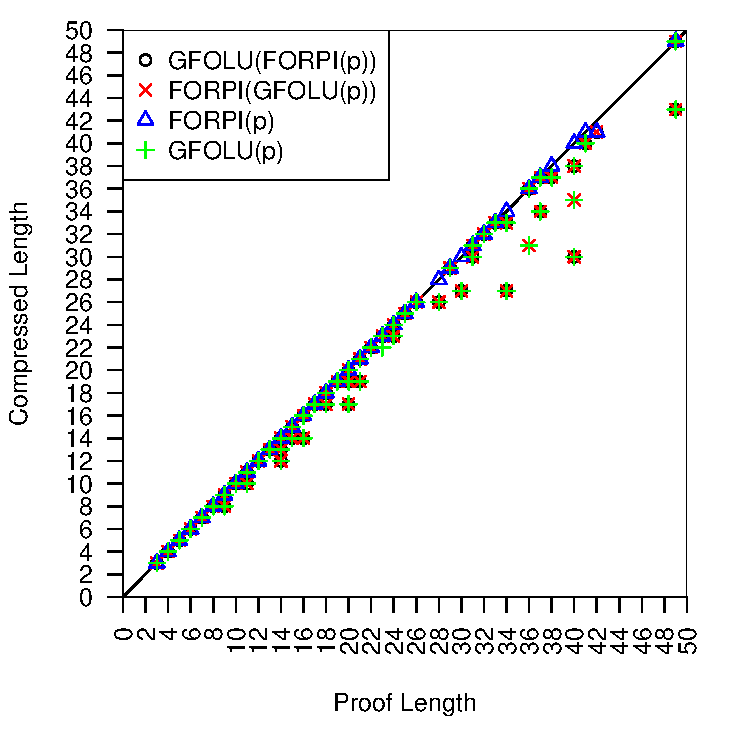
\includegraphics[scale=1]{images/everything-forpi-folu-length_vs_compress_length_all_proofs.pdf}\\
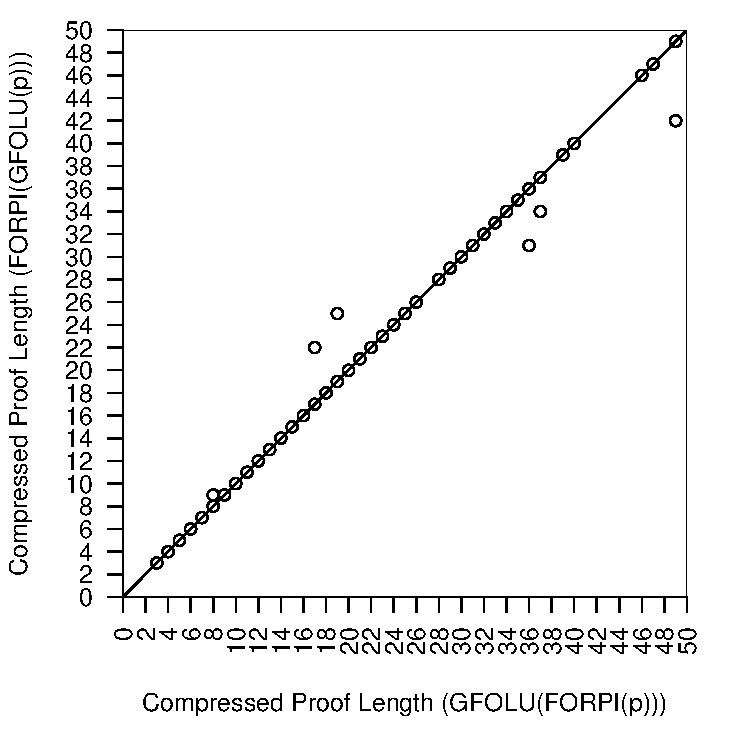
\includegraphics[scale=1]{images/forpi-folu-vs-folu-forpi-length_vs_compress_length_all_proofs.pdf}
\end{column}
\begin{column}{0.65\textwidth}
\begin{itemize}
\item First-order proofs generated by SPASS show some compression by Scala based implementation.
\item Data set is small: only 308 proofs, all of which are short
\item Evaluation with \texttt{GFOLU} \cite{GFOLU}, a first-order variant of \texttt{LowerUnits}, another propositional compression algorithm lifted to first-order logic.
\begin{itemize}
\item Recycle pivots compresses 10x more than lower units in the propositional case
\end{itemize}
\item Algorithm composition may matter less in the first-order case when compared to the propositional case.
\item Quick compression: 40 minutes to generate all proofs, 8 seconds to compress all proofs.
\end{itemize}
\end{column}
\end{columns}
    \end{block}
    

    
          \begin{block}{Future Directions}
    \begin{itemize}
    \item Larger evaluation - more proofs, bigger proofs
    \item Identify properties that would enable all irregular first-order proofs to be compressed
    \item Is it possible to lift other propositional proof compression techniques to first-order logic?
    \end{itemize}
    	\end{block}
    
      \begin{block}{References}
\bibliographystyle{plain}
\bibliography{biblio}
    \end{block}    
        \vfill
  \end{column}
\end{columns}


    
  \end{frame}

\end{document}

